% !TEX program = xelatex
% ---------------------------------------------------------------------------
%  The Hidden Origin  —  a short note
%  Compile with:  xelatex hidden_origin.tex   (twice)
%  Figures: fig1_halving.pdf, fig2_ratios.pdf (figs_halving.py)
%  Exact checks: verify_halving.py
% ---------------------------------------------------------------------------
\documentclass[11pt,a4paper]{article}

\usepackage[margin=2.6cm]{geometry}
\renewcommand{\topfraction}{0.9}\renewcommand{\bottomfraction}{0.8}\renewcommand{\textfraction}{0.07}\renewcommand{\floatpagefraction}{0.8}
\usepackage{amsmath,amsthm,mathtools}
\usepackage{fontspec}
\usepackage{unicode-math}
\setmainfont{Latin Modern Roman}
\setmathfont{Latin Modern Math}
\usepackage{graphicx}
\usepackage{enumitem}
\usepackage[hidelinks]{hyperref}
\usepackage{caption}
\captionsetup{font=small,labelfont=bf}

\theoremstyle{plain}
\newtheorem{theorem}{Theorem}
\newtheorem{proposition}[theorem]{Proposition}
\newtheorem{corollary}[theorem]{Corollary}
\theoremstyle{definition}
\newtheorem{definition}[theorem]{Definition}
\theoremstyle{remark}
\newtheorem{remark}[theorem]{Remark}

\hypersetup{
  pdftitle={The Hidden Origin: halving squares and the start of the Fibonacci spiral},
  pdfauthor={Lluis Garcia Torcal},
  pdfkeywords={Fibonacci spiral, Fibonacci tiling, Holden's lines, spiral similarity, circle of origins, Gaussian integers, 3-4-5 triangle}
}

\begin{document}

\begin{center}
{\LARGE The Hidden Origin\par}
\vspace{0.3em}
{\large Halving squares and the start of the Fibonacci spiral\par}
\vspace{1.2em}
{\large Lluis Garcia Torcal\par}
\vspace{0.3em}
{\small Independent researcher, Sabadell, Spain \quad·\quad ORCID \href{https://orcid.org/0009-0007-8570-2536}{0009-0007-8570-2536}\\ \href{mailto:lluisgarciamusic@gmail.com}{lluisgarciamusic@gmail.com}\par}
\vspace{0.3em}
{\small Version 1, October 2026\par}
\end{center}

\vspace{0.8em}
\begin{abstract}
\noindent The Fibonacci spiral starts abruptly, at a corner of its first square. We run the rule that builds it backwards from that corner, with squares of sides $\tfrac12,\tfrac14,\tfrac18,\dots$. Each new arc continues the one before with the same tangent, the whole lead-in has length $\pi/2$, the length of the spiral's own first arc, and the arcs converge to an exact point, $H'=(\tfrac7{10},-\tfrac1{10})$ when the unit square is centred at $0$. This point is hidden: it is not in the unit square but in the next square of the grid. It is the mirror image of Holden's crossing $H_0=(\tfrac3{10},-\tfrac1{10})$ in the side the two squares share, so it is one of the eight origins of the neighbouring square, the origin of the mirror-image tiling that starts there; it also lies on the circle through the four corners of the unit square. The halving squares and the unit square are one geometric sequence under the spiral similarity $z\mapsto H'-\tfrac{i}{2}(z-H')$, so, as for any such sequence, their centres lie alternately on two perpendicular lines through $H'$ and $H'$ lies on the circle through the corners of every square; here the lines have slopes $7$ and $-\tfrac17$, and the second passes through the centre of the unit square. For a lead-in of any constant ratio $q$ between $0$ and $1$ the limit is known to lie on the circle through the corners of the first square; we write it as the corner turned about the centre by $-2\arctan q$ and show that it is an origin exactly for $q=\tfrac12$ and $q=\tfrac13$, which turn the corner by the two acute angles of the $3$-$4$-$5$ triangle. For $q=1/\varphi$ it is the classical pole of the golden rectangle, which is $\sqrt5\,H_0$ and lies on Holden's line through the centre. All statements are elementary; the rational ones are verified in exact arithmetic.
\end{abstract}

\section{Setting and names}

We use the frame of \cite{origins}. The unit square has its centre at $O=0$ and corners $\pm\tfrac12\pm\tfrac12 i$; points are complex numbers $z=x+iy$, and $E=\tfrac12+\tfrac12 i$ is the top right corner. The Fibonacci tiling is built from the unit square by attaching squares of sides $1,2,3,5,\dots$ below, to the right, above and to the left, in turn, and its spiral is drawn by one rule: in square $k$, of side $s_k$, the arc is the quarter circle of radius $s_k$
\begin{equation}\label{eq:rule}
  \text{about}\quad c_k = P_{k-1} - s_k\, i^{k},\qquad\text{from } P_{k-1}\ \text{to}\ P_k = P_{k-1} + s_k\, i^{k}(i-1),
\end{equation}
starting from $P_0=E$. For $k=1$ this is the arc about the corner $\tfrac12-\tfrac12 i$ from $E$ to $-\tfrac12-\tfrac12 i$, the first arc of the spiral; for $k=2$ it is the arc about the same corner $\tfrac12-\tfrac12i$, now the top right corner of the second square, below the first, and so on. Equivalently $P_k=c_k+s_k\,i^{k+1}$. The centres of the squares lie alternately on Holden's two lines \cite{holden,gardiner}, $x+3y=0$ through $O$ and $3x-y=1$, which cross at Holden's crossing
\[
  H_0=\tfrac3{10}-\tfrac1{10}\,i .
\]
As in \cite{origins}, $\rho=\sqrt{0.1}$ is the \emph{origins unit}, the circle of radius $\rho$ about the centre of a unit square is its \emph{circle of origins}, and the eight points where that circle meets the four diagonal arcs of the square, $(\pm\tfrac3{10},\pm\tfrac1{10})$ and $(\pm\tfrac1{10},\pm\tfrac3{10})$ from its centre, are its \emph{eight origins}, one for each of the eight tilings obtained from the Fibonacci tiling by the symmetries of the square; $H_0$ is one of them. The \emph{unit grid} is the grid of unit squares centred at the points with integer coordinates; its squares are cells of the plane, not tiles of the Fibonacci tiling. We call the cell with centre $1$, which shares the side $x=\tfrac12$ with ours, the \emph{neighbouring square}. A tiling that \emph{starts from} the neighbouring square is one of the eight tilings of \cite{origins} shifted by $1$; it overlaps ours, and its origin is the corresponding origin of the neighbouring square. Finally we call the circle $|z|=\sqrt2/2$ through the four corners of the unit square the \emph{corners' circle}.

The rule \eqref{eq:rule} cannot simply be run backwards with Fibonacci sides: before $1,1$ come $0$ and then $1,-1,2,\dots$, and a square of side $0$ ends the spiral at $E$. To continue it, a choice of sides is needed. The simplest choice keeps the rule and halves the side at each step back.

\section{The halving squares}

\begin{definition}
The \emph{halving squares} are the squares $k=0,-1,-2,\dots$ of sides $s_k=2^{k-1}$, that is $\tfrac12,\tfrac14,\tfrac18,\dots$, placed and drawn by the rule \eqref{eq:rule} run backwards from $P_0=E$:
\[
  P_{k-1}=P_k-s_k\,i^{k}(i-1),\qquad k=0,-1,-2,\dots
\]
Square $k$ has corners $c_k$, $P_k$, $P_{k-1}$ and $P_k+P_{k-1}-c_k$, and the arc in it, about $c_k$, joins $P_{k-1}$ to $P_k$.
\end{definition}

The first halving square ($k=0$) is $[\tfrac12,1]\times[0,\tfrac12]$, against the right side of the unit square; its arc, about $\tfrac12$, runs from $1$ to $E$. At $E$ both this arc and the first Fibonacci arc have their centres straight below $E$ (at $\tfrac12$ and at $\tfrac12-\tfrac12 i$), so they have the same horizontal tangent there and the spiral passes through $E$ without a corner; only the radius changes, from $\tfrac12$ to $1$, as it does at every Fibonacci junction except the first. The next squares are $[\tfrac34,1]\times[-\tfrac14,0]$, $[\tfrac58,\tfrac34]\times[-\tfrac14,-\tfrac18]$, \dots, each against half a side of the one before, winding inwards inside the neighbouring square without overlapping one another or the unit square (Figure~\ref{fig:halving}). They lie in the region covered by the third Fibonacci square, $[\tfrac12,\tfrac52]\times[-\tfrac32,\tfrac12]$: the lead-in is drawn over the tiling, not added to it.

\begin{theorem}[the hidden origin]\label{thm:limit}
The ends $P_k$ of the halving arcs converge to
\[
  H'=\tfrac7{10}-\tfrac1{10}\,i ,
\]
with $P_{-m}-H'=(-\tfrac{i}{2})^{m}(E-H')$, so each step back brings the spiral twice as close to $H'$ and turns it a quarter turn about it. Each arc continues the one before with the same tangent, and the whole lead-in, from $H'$ to $E$, has length $\tfrac\pi2(\tfrac12+\tfrac14+\cdots)=\tfrac\pi2$, the length of the first arc of the spiral.
\end{theorem}

\begin{proof}
The steps $P_k-P_{k-1}=2^{k-1}i^k(i-1)$, $k=0,-1,\dots$, are $\tfrac12(i-1)(-\tfrac{i}{2})^{m}$ with $m=-k$, a geometric series of ratio $-\tfrac i2$. Their sum is $\tfrac12(i-1)/(1+\tfrac i2)=(i-1)/(2+i)=\tfrac15(-1+3i)$, so the limit is $E-\tfrac15(-1+3i)=\tfrac7{10}-\tfrac1{10}i$. The tail after $m$ steps is the same series multiplied by $(-\tfrac i2)^m$, which gives $P_{-m}-H'$. At each junction $P_k$ the radii to the two arcs, $P_k-c_k=s_k\,i^{k+1}$ and $P_k-c_{k+1}=s_{k+1}\,i^{k+1}$, are positive multiples of the same direction, so the two arcs have the same tangent there and lie on the same side of it; this holds for any sides, Fibonacci or halving. The arc of square $k$ is a quarter circle of radius $s_k$, of length $\tfrac\pi2 s_k$, and $\sum_{k\le0}s_k=1$.
\end{proof}

\begin{proposition}[where $H'$ is]\label{prop:where}
\begin{enumerate}[label=(\alph*),itemsep=1pt]
\item $H'$ is the mirror image of Holden's crossing $H_0$ in the side $x=\tfrac12$ shared by the unit square and the neighbouring square.
\item $|H'-1|=\rho$: $H'$ lies on the circle of origins of the neighbouring square and is one of its eight origins, namely the origin (Holden's crossing) of the mirror-image tiling that starts from the neighbouring square, the image of our tiling under the reflection in $x=\tfrac12$.
\item $|H'|=\sqrt2/2$: $H'$ lies on the corners' circle of the unit square.
\end{enumerate}
\end{proposition}

\begin{proof}
(a) The reflection is $x+iy\mapsto(1-x)+iy$, and $1-\tfrac3{10}=\tfrac7{10}$. (b) $|H'-1|^2=\tfrac9{100}+\tfrac1{100}=\tfrac1{10}$. The reflection in $x=\tfrac12$ maps the unit square to the neighbouring square, its circle of origins to theirs, and the tiling with its Holden crossing $H_0$ to a mirror-image tiling with Holden crossing $H'$. (c) $\tfrac{49}{100}+\tfrac1{100}=\tfrac12$.
\end{proof}

So the spiral, followed backwards from its first corner, does not end in its own square: it ends at a point of the neighbouring square, at the origin of that square's mirror tiling. It is not one of the unit square's own eight origins; it is found on the circle of origins of the square next to it.

\begin{figure}[t]
\centering
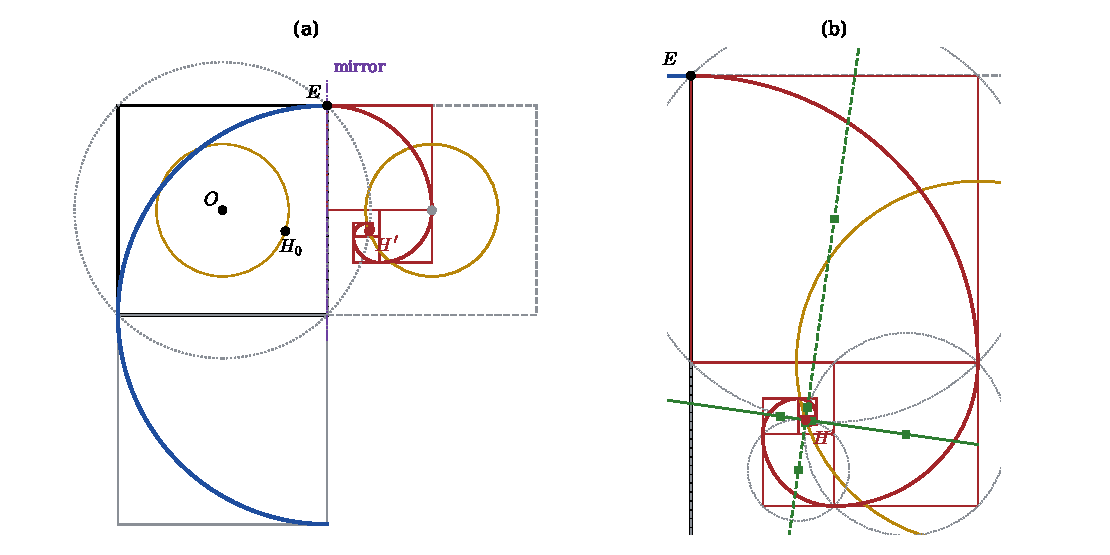
\includegraphics[width=\textwidth]{fig1_halving.pdf}
\caption{(a) The first two arcs of the Fibonacci spiral (blue) and the halving squares and their arcs (red), which lead into the corner $E$ from the hidden origin $H'$. $H'$ is the mirror image of Holden's crossing $H_0$ in the shared side (purple), lies on the circle of origins (gold) of the neighbouring square (dashed), and on the corners' circle of the unit square (dotted); the unit square's own circle of origins, through $H_0$, is also shown. (b) Enlarged: the centres of the halving squares (green) lie alternately on two perpendicular lines through $H'$, of slopes $7$ (dashed) and $-1/7$; the line of slope $-1/7$ continues to $O$ (outside the panel). $H'$ lies on the circle through the corners of every halving square (dotted, first three shown).}
\label{fig:halving}
\end{figure}

\section{One similarity: centres and lines}

\begin{theorem}\label{thm:centres}
Let $f(z)=H'-\tfrac i2\,(z-H')$, the quarter turn clockwise about $H'$ followed by halving.
\begin{enumerate}[label=(\alph*),itemsep=1pt]
\item $f$ maps the unit square, with its arc, onto the first halving square, with its arc, and each halving square, with its arc, onto the next. In particular $f(E)=1$ and $f(-\tfrac12-\tfrac12i)=E$.
\item Writing square $-1$ for the unit square ($s=1$, centre $O$) and numbering the halving squares $j=0,1,2,\dots$ (side $s_j=2^{-j-1}$, so square $j$ is square $k=-j$ above), the centres are
\[
  C_j = H' + \frac{s_j}{10}\,(1+7i)\,(-i)^{j},\qquad j=-1,0,1,2,\dots
\]
\item The centres $C_0,C_2,C_4,\dots$ lie on the line of slope $7$ through $H'$, and $O=C_{-1}$, $C_1,C_3,\dots$ on the perpendicular line of slope $-\tfrac17$ through $H'$, which is the line $x+7y=0$ through $O$.
\item $|C_j-H'|=s_j/\sqrt2$: $H'$ lies on the circle through the four corners of every square of the sequence, the unit square included.
\end{enumerate}
\end{theorem}

\begin{proof}
(a) $f(E)=\tfrac7{10}-\tfrac1{10}i-\tfrac i2(-\tfrac15+\tfrac35 i)=1$ and $f(-\tfrac12-\tfrac12i)=\tfrac7{10}-\tfrac1{10}i-\tfrac i2(-\tfrac65-\tfrac25 i)=E$; and $f(\tfrac12-\tfrac12i)=\tfrac12$, the centre of the first halving arc. A similarity that maps the centre and both ends of a quarter circle to the centre and ends of another maps the one onto the other, and the square on that arc onto the square on the image. At every later step: by Theorem~\ref{thm:limit}, $f(P_k)=P_{k-1}$ for all $k\le1$, since $f$ multiplies $P_k-H'$ by $-\tfrac i2$ and $f(P_1)=E$; and since $f(z+w)=f(z)-\tfrac i2 w$ and $s_{k-1}=\tfrac12 s_k$, $f(c_k)=f(P_{k-1})+\tfrac i2 s_k\,i^{k}=P_{k-2}-s_{k-1}\,i^{k-1}=c_{k-1}$. (b) $f(O)=H'(1+\tfrac i2)=\tfrac34+\tfrac14i=C_0$, and $C_{-1}=O=H'+\tfrac1{10}(1+7i)\,i$ since $(1+7i)\,i=-7+i$. Each application of $f$ multiplies $C_j-H'$ by $-\tfrac i2$, which is the step from $j$ to $j+1$ in the formula. (c) The two lines are perpendicular because $f$ turns by a quarter turn, as for any quarter-turn similarity (for golden squares this is in Hoggatt and Alladi \cite{hoggatt}); their slopes are those of $1+7i$, namely $7$, and of $(1+7i)(-i)=7-i$, namely $-\tfrac17$. The line of slope $-\tfrac17$ through $H'$ is $x+7y=\tfrac7{10}-\tfrac7{10}=0$. (d) $|1+7i|=\sqrt{50}$, so $|C_j-H'|=s_j\sqrt{50}/10=s_j/\sqrt2$, half the diagonal of square $j$. (That the limit point of whirling squares of any constant ratio lies on the circumcircle of every square was proved by Silveira \cite[Thm.~2.6]{silveira}.)
\end{proof}

\begin{remark}[Holden's lines and the new lines]\label{rem:gauss}
Holden's lines have directions $1+3i$ and $3-i=-i(1+3i)$; the new lines have directions $1+7i$ and $7-i=-i(1+7i)$. In Gaussian integers
\[
  1+3i=(1+i)(2+i),\qquad 1+7i=(1+i)(4+3i),\qquad 4+3i=i\,(2-i)^2 :
\]
both are the diagonal direction $1+i$ turned, Holden's by the angle of $2+i$, $\arctan\tfrac12=26.57^\circ$, and the new one by the angle of $4+3i$, $\arctan\tfrac34=36.87^\circ$, one of the two acute angles of the $3$-$4$-$5$ triangle that separate consecutive origins in \cite{origins}. Both lines through $O$, Holden's $x+3y=0$ and the new $x+7y=0$, pass through an origin: $H_0$, an origin of the unit square, and $H'$, an origin of the neighbouring square.
\end{remark}

\section{Other ratios}

The halving ratio is a choice. Any constant ratio $q$ with $0<q<1$ gives a lead-in by the same rule, with sides $q,q^2,q^3,\dots$; its first square is $[\tfrac12,\tfrac12+q]\times[\tfrac12-q,\tfrac12]$, against the right side of the unit square, and its arcs continue the first arc with the same tangent at every junction. For $q\le1/\varphi$ the squares fit against one another without overlapping; for $q=1/\varphi$ they are the whirling squares that, with the unit square, fill the golden rectangle $[-\tfrac12,\tfrac12+\tfrac1\varphi]\times[-\tfrac12,\tfrac12]$. For $q>1/\varphi$ the squares overlap (since $q^2+q^3>q$), and only the curve and its limit behave as below.

\begin{theorem}\label{thm:ratios}
The lead-in of ratio $q$, $0<q<1$, converges to
\[
  L(q)=E\,\frac{1-iq}{1+iq},
\]
the corner $E$ turned clockwise about $O$ by the angle $2\arctan q$. All these limits lie on the corners' circle (as Silveira proved for any ratio \cite[Cor.~2.7]{silveira}), on its quarter from $E$ to $\tfrac12-\tfrac12i$, inside the neighbouring square. The lead-in has length $\tfrac\pi2\,q/(1-q)$, which equals the length $\tfrac\pi2$ of the first arc exactly when $q=\tfrac12$.
\end{theorem}

\begin{proof}
The steps $P_k-P_{k-1}=s_k\,i^k(i-1)$, $k=0,-1,\dots$, with $s_k=q^{1-k}$, form a geometric series with first term $q(i-1)$ and ratio $-iq$. So $L=E-q(i-1)/(1+iq)$, and since $i-1=2iE$, $L=E\,(1+iq-2iq)/(1+iq)=E(1-iq)/(1+iq)$. For real $q$, $|1-iq|=|1+iq|$, so $|L|=|E|$, and $(1-iq)/(1+iq)$ has argument $-2\arctan q$, which lies between $0$ and $-90^\circ$. The arc lengths are $\tfrac\pi2(q+q^2+\cdots)$.
\end{proof}

\begin{corollary}[which ratios end at an origin]\label{cor:origins}
Among all ratios $0<q<1$, the limit $L(q)$ is an origin of a square of the unit grid exactly for
\[
  q=\tfrac12:\ \ L=H'=\tfrac7{10}-\tfrac1{10}i \qquad\text{and}\qquad q=\tfrac13:\ \ L=\tfrac7{10}+\tfrac1{10}i .
\]
They turn $E$ by $\arctan\tfrac43=53.13^\circ$ and $\arctan\tfrac34=36.87^\circ$, since $(1-\tfrac i2)/(1+\tfrac i2)=\tfrac{3-4i}5$ and $(1-\tfrac i3)/(1+\tfrac i3)=\tfrac{4-3i}5$. These two points are exactly where the corners' circle of the unit square meets the circle of origins of the neighbouring square. The limit for $q=\tfrac13$ is the image of $H_0$ under the half turn about the midpoint $\tfrac12$ of the shared side: the origin of the half-turned tiling that starts from the neighbouring square.
\end{corollary}

\begin{proof}
The origins of the squares of the unit grid are the points whose coordinates, in tenths, are $\equiv\pm3$ and $\equiv\pm1 \pmod{10}$ in either order. On the corners' circle, $x^2+y^2=\tfrac12$, the points with coordinates in tenths $(a,b)$ have $a^2+b^2=50$, so $(a,b)$ is $(\pm7,\pm1)$, $(\pm1,\pm7)$ or $(\pm5,\pm5)$; the last four are the corners and are not origins. Of the eight others only $(7,\pm1)$ lie on the open quarter of Theorem~\ref{thm:ratios}, and since the angle $2\arctan q$ increases with $q$, each is reached by exactly one ratio, $q=\tfrac12$ and $q=\tfrac13$. Solving $|z|^2=\tfrac12$, $|z-1|^2=\tfrac1{10}$ gives $2x-1=\tfrac25$, $x=\tfrac7{10}$, $y=\pm\tfrac1{10}$. Finally $1-(\tfrac3{10}-\tfrac1{10}i)=\tfrac7{10}+\tfrac1{10}i$.
\end{proof}

Thus the two ratios that end at an origin end at the images of $H_0$ under the two symmetries that swap the unit square and the neighbouring square and keep their shared side: the mirror in that side ($q=\tfrac12$) and the half turn about its midpoint ($q=\tfrac13$). Only the halving lead-in has the length of the first arc.

\begin{proposition}[the golden lead-in]\label{prop:golden}
For $q=1/\varphi$, $\varphi=(1+\sqrt5)/2$, the limit, which is the classical pole of the golden rectangle formed by the unit square and its golden lead-in, is
\[
  L(1/\varphi)=\sqrt5\,H_0=\tfrac{3\sqrt5}{10}-\tfrac{\sqrt5}{10}\,i ,
\]
on Holden's line $x+3y=0$ through $O$ and $H_0$, at $\sqrt5\,\rho$ from $O$. The turn is $2\arctan(1/\varphi)=\arctan 2=63.43^\circ$.
\end{proposition}

\begin{proof}
$(\varphi-i)/(\varphi+i)=(\varphi-i)^2/(\varphi^2+1)=\varphi(1-2i)/(\varphi+2)$, using $\varphi^2=\varphi+1$. Then $E\,\varphi(1-2i)/(\varphi+2)=\tfrac12(3-i)\,\varphi/(\varphi+2)$, and $\varphi+2=\tfrac{5+\sqrt5}2=\sqrt5\,\varphi$, so the limit is $(3-i)/(2\sqrt5)=\sqrt5\,(\tfrac3{10}-\tfrac1{10}i)$. For the angle, $\tan 2a=2t/(1-t^2)=2$ with $t=1/\varphi$, since $1-1/\varphi^2=1/\varphi$.
\end{proof}

\begin{figure}[t]
\centering
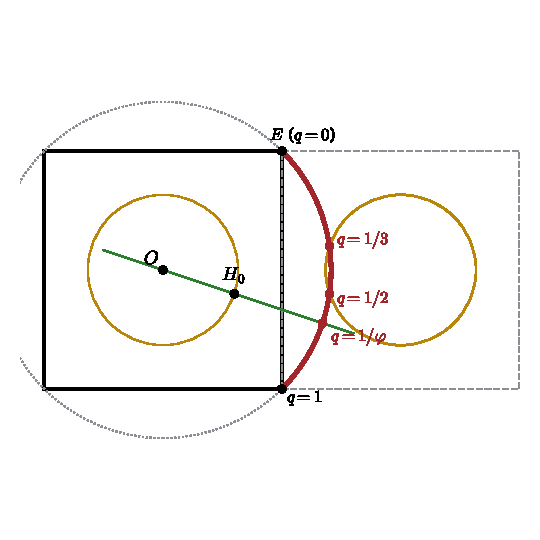
\includegraphics[width=0.46\textwidth]{fig2_ratios.pdf}
\caption{The limits $L(q)$ of the lead-ins of ratio $0<q<1$ (red) run along the corners' circle (dotted) from $E$ towards the corner below it (the end values $q\to0$ and $q\to1$). Only $q=1/3$ and $q=1/2$ end on the circle of origins of the neighbouring square (gold, right), at its two origins $\tfrac7{10}\pm\tfrac1{10}i$. The ratio $q=1/\varphi$ ends at $\sqrt5\,H_0$, on Holden's line through $O$ and $H_0$ (green); the gold circle on the left is the unit square's own circle of origins, through $H_0$.}
\label{fig:ratios}
\end{figure}

\section{Further remarks}

\begin{enumerate}[leftmargin=*,itemsep=0pt,topsep=2pt]
\item The same holds for each of the eight tilings of \cite{origins}: the symmetry of the square that maps our tiling to another maps its halving squares and its hidden origin to that tiling's, so each of the eight spirals has a hidden origin in one of the four neighbouring squares, at the mirror image of its own origin in the side against which its first halving square lies.
\item The Fibonacci tiling itself is not self-similar (the ratios $F_{k+1}/F_k$ only tend to $\varphi$), so it has no fixed point of this kind; the halving lead-in is exactly self-similar, and $H'$ is its centre. Squares shrinking by a constant ratio and their pole are classical (for the golden rectangle, the well-known pole of the golden spiral). For any ratio the pole lies on the circumcircle of every square and of the first square \cite{silveira}, and for in-winding golden squares the centres lie on two perpendicular lines through it \cite{hoggatt}; with ratio $\tfrac12$ and the unit square as first square, Silveira's formula for the pole \cite[Thm.~2.3]{silveira} gives $H'$ (and with ratios $\tfrac13$ and $1/\varphi$ it gives $\tfrac7{10}+\tfrac1{10}i$ and $\sqrt5\,H_0$). What we have not found in the literature is the reading of this point as an origin of the neighbouring square, the mirror image of Holden's crossing; the ratio $\tfrac13$ and the half turn; the lines of slopes $7$ and $-\tfrac17$ through $O$; and the golden pole on Holden's line.
\item In the author's Spiral Workbench the halving lead-in is drawn for all eight spirals, and $H'$, where the spiral starts, is one of the centres about which the spirals can be turned: \url{https://lluisgarcia.github.io/The-Pentametric-Cycle/spiral-workbench/}.
\item Exact checks: \texttt{verify\_halving.py} (the rational statements in exact Gaussian-rational arithmetic, the golden case numerically); figures: \texttt{figs\_halving.py}. Repository: \url{https://github.com/lluisgarcia/The-Pentametric-Cycle}.
\end{enumerate}

\paragraph{Acknowledgements and use of AI.} The idea of continuing the spiral inwards by halving the squares, the observation that it ends at the origin of the neighbouring mirror square, and the name are the author's, found in the Spiral Workbench (an interactive page built for this study with Claude Code). Claude (Anthropic, Opus 5.5) was used to compute the limit and the lines in exact arithmetic, to find the general form for other ratios, to search the literature, to prepare the figures and to help draft the text, and two further independent Claude sessions checked the statements and the references; the author checked and approved every statement. Licence: CC BY 4.0 for this note, MIT for the Python scripts.

{\footnotesize\begin{thebibliography}{9}\setlength{\itemsep}{0pt}
\bibitem{holden} H.~L. Holden, Fibonacci tiles, \emph{The Fibonacci Quarterly} \textbf{13} (1975) 45--49.
\bibitem{gardiner} T. Gardiner, 68.15 The Fibonacci spiral, \emph{The Mathematical Gazette} \textbf{68} (1984) 120, \href{https://doi.org/10.2307/3615922}{doi:10.2307/3615922}.
\bibitem{hoggatt} V.~E. Hoggatt, Jr.\ and K. Alladi, In-winding spirals, \emph{The Fibonacci Quarterly} \textbf{14} (1976) 144--146.
\bibitem{silveira} C. Silveira, Notes on approximate golden spirals with whirling squares, preprint (2013), \href{https://arxiv.org/abs/1308.5941}{arXiv:1308.5941}.
\bibitem{origins} L. Garcia Torcal, \emph{The Origin of Origins}, note, Zenodo (2026), \href{https://doi.org/10.5281/zenodo.23486276}{doi:10.5281/zenodo.23486276}.
\end{thebibliography}}

\end{document}
